% \subfloat[Structured data]{%
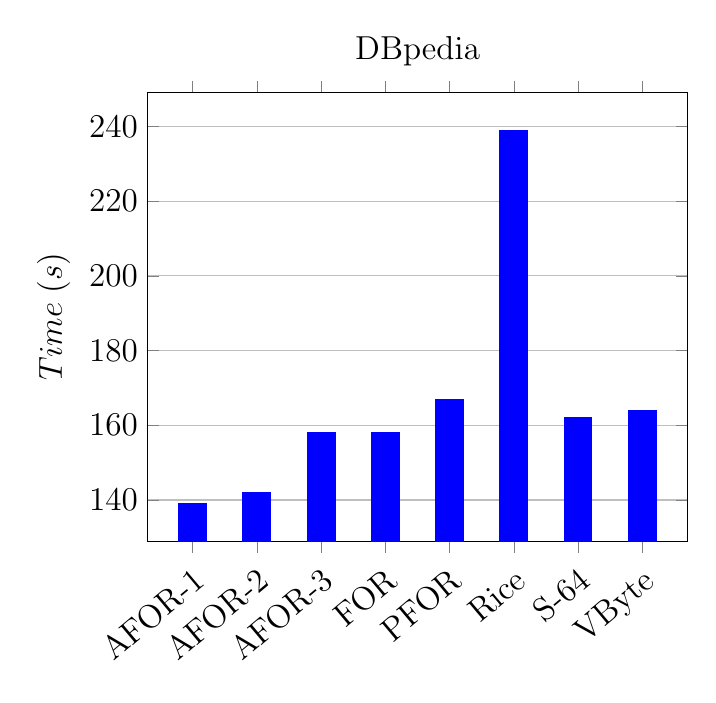
\begin{tikzpicture}[baseline]
\begin{axis}[
ylabel=$Time \; (s)$,
x tick label style={rotate=40, anchor=north east},
xtick={1,...,8},
xticklabels={AFOR-1, AFOR-2, AFOR-3, FOR, PFOR, Rice, S-64, VByte},
legend style={at={(0.5,1.13)}, anchor=north, legend columns=-1},
label style={font=\large},
tick label style={font=\large},
title style={font=\large},
ybar,
ymajorgrids=true,
bar width=10pt,
title={DBpedia},
%enlargelimits=0.15,
]
\addplot[draw=blue,fill=blue]
coordinates {(1, 139) (2, 142) (3, 158) (4, 158) (5, 167) (6, 239) (7, 162) (8, 164)};
\end{axis}
\end{tikzpicture}%
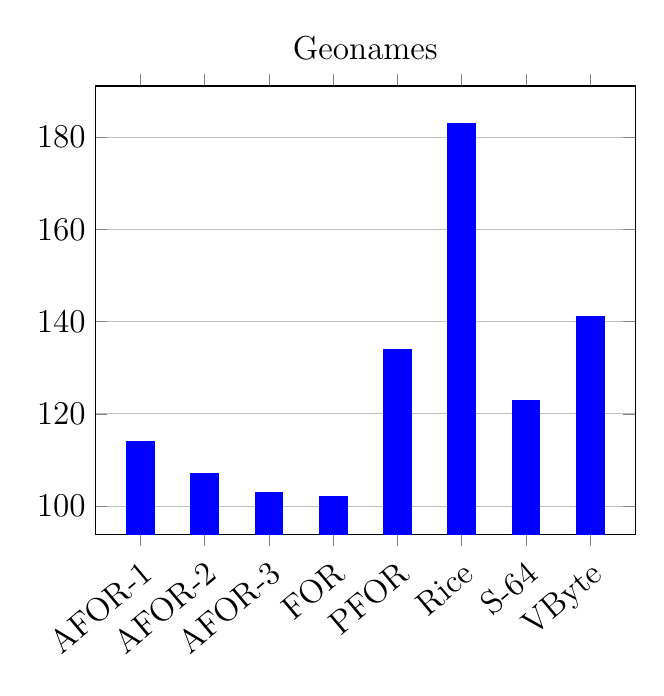
\begin{tikzpicture}[baseline]
\begin{axis}[
x tick label style={rotate=40, anchor=north east},
xtick={1,...,8},
xticklabels={AFOR-1, AFOR-2, AFOR-3, FOR, PFOR, Rice, S-64, VByte},
legend style={at={(0.5,1.13)}, anchor=north, legend columns=-1},
label style={font=\large},
tick label style={font=\large},
title style={font=\large},
ybar,
ymajorgrids=true,
bar width=10pt,
title={Geonames},
%enlargelimits=0.15,
]
\addplot[draw=blue,fill=blue]
coordinates {(1, 114) (2, 107) (3, 103) (4, 102) (5, 134) (6, 183) (7, 123) (8, 141)};
%\legend{Blog}
\end{axis}
\end{tikzpicture}
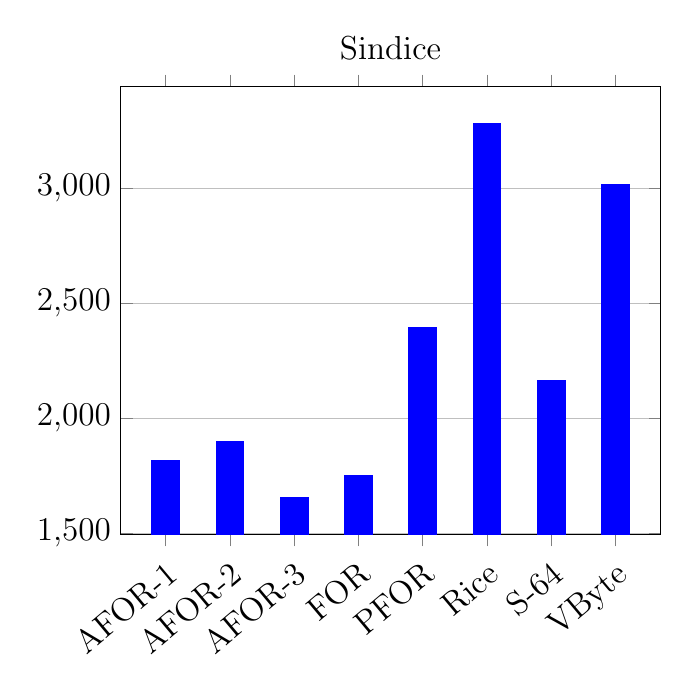
\begin{tikzpicture}[baseline]
\begin{axis}[
x tick label style={rotate=40, anchor=north east},
xtick={1,...,8},
xticklabels={AFOR-1, AFOR-2, AFOR-3, FOR, PFOR, Rice, S-64, VByte},
legend style={at={(0.5,1.13)}, anchor=north, legend columns=-1},
label style={font=\large},
tick label style={font=\large},
title style={font=\large},
ybar,
ymajorgrids=true,
bar width=10pt,
title={Sindice},
%enlargelimits=0.15,
]
\addplot[draw=blue,fill=blue]
coordinates {(1, 1816) (2, 1900) (3, 1656) (4, 1749) (5, 2396) (6, 3281) (7, 2163) (8, 3018)};
%\legend{Blog}
\end{axis}
\end{tikzpicture}
% }